\documentclass[11pt, a4paper]{article}

\usepackage[utf8]{inputenc}
\usepackage{authblk}
\usepackage{titlesec}


% Maths tools
\usepackage[tbtags]{amsmath}
\usepackage{amssymb}

% Margin
\usepackage[margin=2.9cm]{geometry}

% Line numbers
\usepackage{lineno}

% Spacing
\usepackage{setspace}
\doublespacing

% Enumeration
\usepackage{enumerate}% http://ctan.org/pkg/enumerate
\usepackage{enumitem}


% indentation
\setlength\parindent{10pt}
\setlength{\parskip}{5pt}

% Figures
\usepackage{graphicx}
\usepackage{caption}
\usepackage{subcaption}
\usepackage{epstopdf}
\usepackage{float}
\renewcommand{\thefigure}{\textbf{\arabic{figure}}}
\renewcommand{\figurename}{\textbf{Figure}}


%table
\usepackage{multirow}% http://ctan.org/pkg/multirow
\usepackage{hhline}
\usepackage[table]{xcolor}

\usepackage{authblk}


% References
\usepackage[round]{natbib}
\bibliographystyle{ecology_letters2.bst}

\usepackage{color, xcolor,soul}
%\definecolor{blau}{RGB}{168,221,181}
\definecolor{blau}{RGB}{236,226,240}
\soulregister\cite7
\soulregister\citenum7
\soulregister\citep7
\soulregister\citealt7
\soulregister\citealp7
\soulregister\citet7
\soulregister\ref7

% References and links
\PassOptionsToPackage{hyphens}{url}\usepackage[colorlinks=true,linkcolor=magenta, citecolor=magenta]{hyperref}

%Margin notes
\usepackage{marginnote}
% Foot note distance with text
\usepackage[symbol]{footmisc}
\renewcommand{\thefootnote}{\fnsymbol{footnote}}
\setlength{\skip\footins}{0.75cm}

%Define colour
\DeclareRobustCommand{\hlc}[1]{{\sethlcolor{blau}\hl{#1}}}

%subsubsection format
\titleformat*{\subsubsection}{\large\it}

\makeatletter
\renewcommand\AB@affilsepx{; \protect\Affilfont}
\makeatother

%Title paper
\title{\vspace{-1cm}
Model simplicity breeds contempt: using simple models to answer basic questions on species' distributions}
\author[1,*]{\normalsize Bernat Bramon Mora}
\author[1]{\normalsize Jake M.\ Alexander}
\affil[1]{\footnotesize Institute of Integrative Biology, ETH Zürich, Zürich, Switzerland}
\affil[*]{\footnotesize  bernat.bramon@gmail.com}

\renewcommand\Authands{ and }
\date{}

\begin{document}
\maketitle
\linenumbers

\section*{Abstract}
We know a lot about the factors that could theoretically influence species' distributions, and a rapidly growing body of research have been primarily focused on trying to untangle some of such biotic and abiotic predictors---with an increasing effort placed in improving the predictive power of statistical models. However, much less is known about how species' distributions compare to each other. Here, we use a conceptually more conservative approach to instead understand and compare basic aspects regarding the shape of species' distribution along environmental gradients.

\section*{Introduction}

%Consider testing tails of distribution? I would use the Cauchy or generalized normal distribution for heavy tail distribution without skewness; and I would use an exponentially modified Gaussian distribution with heavy tails for a skew distribution with heavy tails. 

One of the central goals of ecology is to understand the ways species are distributed across space and time (ref). Over the last two decades, ecologists have developed multiple distribution models to try to untangle the factors that play a role in defining such distributions \citep{guisanPredictiveHabitatDistribution2000, more}. These models estimate species' realized niches using several covariates, including environmental variables \citep{Guisan}, species ecological traits' \citep{pollockRoleFunctionalTraits2012} and phylogenetic relations \citep{ivesGeneralizedLinearMixed2011}. More recently, some of the focus have shifted towards approaches that estimate and account for biotic factors, such as competitive or facilitative relationships between species \citep{ovaskainenHowMakeMore2017}. The idea is that by untangling the ways in which such biotic and abiotic factors shape species' distributions, we can gain a mechanistic understanding on how ecological communities are established and change over time. However, while these factors can increase the predictive performance of some of the models \citep{norbergComprehensiveEvaluationPredictive2019}, the interpretation of the corresponding parameter estimates has been often questioned \citep{gotelliEmpiricalBayesApproach2010, harrisInferringSpeciesInteractions2016, thurmanTestingLinkSpecies2019}. This was best illustrated by \citet{blanchetCooccurrenceNotEvidence2020}, who used basic statistical arguments to highlight the artefactual nature of the link between co-occurrence and species' ecological interactions drawn by some distribution models.
% Other references for biotic interaction=bad: dormannBioticInteractionsSpecies2018

The value of gaining a mechanistic understanding of species' distributions is unquestionable (ref), with several studies highlighting the importance of factors such as biotic interactions and species' dispersal ability in setting their range limits \citep{wiszRoleBioticInteractions2013, pollockUnderstandingCooccurrenceModelling2014, neuschulzBioticInteractionsSeed2018}. That said, a lot can be learned from taking a phenomenological approach, focussing instead on the description of basic properties of species' realized niches. For example, the study of species' range sizes along environmental gradients can reveal general biodiversity patterns that are crucial from a conservation and management perspective \citep{stevensElevationalGradientAltitudinal1992}. Differences in species' responses to the environment could shed light on how climatic processes and historical contingencies have shaped their distributions \citep{rohdeLatitudinalGradientsSpecies1992, more in Rapoport}. Other properties, such as the skewness of species' distributions, can also reveal general underlying processes regarding species' physiological tolerance to different environmental conditions \citep{kaufmanDiversityNewWorld1995}. More generally, understanding the shape of species' realized niches and the extend to which these vary across species is a crucial issue in ecology and biogeography (ref); however, we do not have an effective way to parsimoniously compare the realized niches of many species. Indeed, there is no general agreement on the shape of species' distributions (ref).

Many ecological textbooks (ref) assume the shape of species distributions to be unimodal and symmetric, but some have warned that empirical distributions can take many different forms \citep{austinModelsAnalysisSpecies1987, austin2002spatial}. In practice, distribution frameworks often use logistic regressions with a linear relationship between covariates (but see XX and YY). This is useful because it simplifies the optimization process, but it comes with several statistical shortcomings. First and foremost, such response curve and the linear relationship between covariates often comes with a set of implicit mathematical constrains that might not be biologically justified. From a purely statistical perspective, if all that we are willing to assume is that species occupy finite geographic ranges---i.e. their probability distributions have finite variance---the most conservative statistical approach is to model these as a Gaussian distributions \citep{frankCommonPatternsNature2009}. This is rarely the starting point in most statistical frameworks that study general biodiversity patterns (but see ref), choosing to use instead Gaussian-logit response curves (refs). Other factors might then condition species distributions to showcase heavy-tails or a skewed shapes, revealing interesting ecological processes shaping biodiversity patterns \citep{austinNonlinearSpeciesResponse1976, minchinEvaluationRelativeRobustness1987}. Second, the aforementioned structural constrains also limit our ability to include any prior information to our parameter estimates. Observations on species' geographic variation and optimal climatic conditions have long been documented, with extensive databases compiled by botanists and field ecologists documenting basic knowledge on species' realized niches (e.g. \citealt{landoltFloraIndicativaOkologische2010}). That said, this information is rarely accounted for in most modelling approaches, mainly because there is not a straightforward way to feed this information into the parameters of a linear model (\citealt{scherrerEcologicalIndicatorValues2019}; but see \citealt{terbraakWeightedAveragingLogistic1986}). Finally, and perhaps most importantly, a direct biological interpretation of parameter estimates in linear models becomes increasingly difficult as one moves from unimodal and symmetric distributions \citep{jamilGeneralizedLinearMixed2013, terbraakWeightedAveragingLogistic1986} to skewed distributions \citep{huismanHierarchicalSetModels1993}, making the tests of hypothesis on global biodiversity patterns particularly challenging. For example, \citet{huismanHierarchicalSetModels1993} proposed several non-linear models to characterize several features of species' response curves; however, species' environmental indicator values, range size or distribution skewness are difficult to capture following these model structures.

% From Ana Norberg: Each statistical modeling method is based on different assumptions that can be viewed as hypotheses about how ecological communities are structured
% While many ecological textbooks (Begon et al., 1990, Giller, 1984, Krebs, 1994)
%Niche theory predicts that species occurrence and abundance show non-linear, unimodal relationships with respect to environmental gradients (Austin, 1987; Palmer & Dixon, 1990; Whittaker, 1967)
%\citet{} showed that bell curves are not universal response curves in vegetation data, with distributions often presenting skewed responses, and some modelling techniques try to account for this asymmetry in species distributions.

The field of ecology has quickly moved towards mechanistic and process-based approaches to understand species' distributions \citep{wartonManyVariablesJoint2015}. This has resulted in a plethora of models accounting for several biotic and abiotic factors into the predictions of species co-occurrence. Here, we instead rethink traditional modelling approaches and develop a conceptually simple---and yet statistical and computationally complex---statistical framework to revisit some classic hypothesis in ecology and biogeoraphy. In particular, we develop a Bayesian hierarchical model that accounts for all prior information that we have regarding the distribution of alpine plant species along an elevation gradient in the Swiss Alps, including expert knowledge on species environmental indicator values, range sizes, and plant physiology. We start by considering species' response curves as Gaussian distributed, and then we adapt our model to allow for skewed and long-tailed distributions. Using this statistical framework, we are able to compare the basic properties of the realized niches of multiple species, testing for the existence of general biogeographical patterns. First, we test for the Rapopor's rule, which predicts a positive relationship between range size and elevation \citep{stevensElevationalGradientAltitudinal1992}. While this pattern has been largely studied for multiple systems and across gradients \citep{mccainElevationalRapoportRule2013}; contrasting evidence suggests this rule not to be pervasive across species \citep{ribasRapoportEffectWidespread2006, bhattaraiCanRapoportRule2006, mccainElevationalRapoportRule2013}. Our results not only allow us to properly test the existence of this geographical pattern, but they also showcase variation in how different types of species, such as native or neophytes, might respond to an environmental gradient. Second, we study whether or not species' distributions show steeper declines towards stressful conditions, testing the so-called abiotic stress limitation hypothesis (ref). \citet{normandImportanceAbioticStress2009} tested this for vegetation data using \citep{huismanHierarchicalSetModels1993}'s statistical models for several independent species, finding no clear support for such a hypothesis. Our results are able to shed light on this geographical pattern as well as to highlight the degree to which different species will showcase different levels of decline towards stressful conditions. Specifically, we are able to link plant physiological traits to the skewness of their distributions. Overall, we use models that is solely constrained by the empirical information that we truly have regarding a particular system, relaxing as much as possible the structural constrains of the statistical framework. Using these model, we are able uncover the shape of empirical plant distributions and answer fundamental questions regarding the way systems of many species are distributed along environmental gradients.



%%%%%%%%%%%%%%%%%%%%%%%FINAL



% To decide among modelling approaches, we first need to agree on what we know about the system. We know that species occupy a geographic range; therefore, we know that their distributions have finite variance. Indeed, observations on species' geographic variation and optimal climatic conditions have been long documented, with extensive databases compiled by botanists and field ecologists documenting basic knowledge on species' distributions. One could point out that we also know that many other factors might influence species' presence/absence---e.g. the influence of the aforementioned biotic interactions among species. However, we do not necessarily have an intuition of how exactly these factors will influence the shape of species' distributions. Therefore, if all we truly knew about a species' distribution was that they have finite variance, the most conservative assumption and the safest bet---i.e. the one with the largest entropy---is that such distribution is a Gaussian.


%The strength of climate as a range limiting factor will becrucial for the extent to which species will retract from theirsouthern range margins and expand northwards under global warming. occurrence of a species along an environmentalgradient may primarily be limited by its physiological tolerancetowards the abiotically more stressful conditions, while otherfactors, such as biotic interactions, may assume a greater roletowards less stressful conditions (Connell, 1961; Austin, 1990;Brown  et al. , 1996); hereafter referred to as the asymmetricabiotic stress limitation (AASL) hypothesis.

%abiotic stress is generally thought to increasetowards high latitudes and altitudes and to decrease in importancetowards the equatorial lowlands, where biotic interactions havebeen argued to increase in importance (Dobzhansky, 1950;Kaufman, 1995). Accordingly, a geographical prediction of theAASL hypothesis is that abiotic stress may be most importantin upper-latitudinal and upper-altitudinal range boundaries(MacArthur, 1972; Brown  et al. , 1996), but this has received littlestudy. Loehle (1998) suggested that the northern and southernrange limits of North American tree species are determined bycold tolerance and competitive ability, respectively. Similarly,abiotic stress appears to determine the upper-altitudinal rangelimit for some mountainous plant species, while biotic interactionsmay determine the lower limit (Guisan  et al ., 1998; Bruelheide &Scheidel, 1999; Vetaas, 2002). A second aspect of the AASL hypothesis proposes that theshape of species response curves vary along an environmentalgradient: species that occur under the physiologically moststressful conditions show skewed responses with a steep declinetowards the stressful conditions, while species that occur underless stressful conditions show symmetric responses (Austin,1990; also cf. Austin  et al ., 1994; Austin & Gaywood, 1994;Rydgren  et al. , 2003). In line with this, Kaufman (1995) suggeststhat the degree to which a species’ poleward range boundary islimited by abiotic stress increases the further north the species isdistributed. Analogously, we expect increasing stress limitationwith increasing elevation

% Guisan found no evidence of that. 
% No support for Kaufman’s (1995) geographical prediction ofthe AASL hypothesis,

 %There is not an easy way to untangle the true shape of species' distributions, as this shape is likely to showcase idiosyncrasies at the species level and across systems. The aim of this work, it is not to answer these questions nor to provide a general approach that accommodates such idiosyncrasies. Instead, we want to use a model that is solely constrained by the empirical information that we truly have regarding a particular system, relaxing as much as possible the structural constrains of the statistical framework. Then, we want to use this model to answer basic aspects regarding the way systems of many species are distributed along an environmental gradient. 


%%%%%%%%%%%%%%% KEY PAPERS AND IDEAS REGARDING HYPOTHESES #################
% EXPLAIN WHY KNOWING THIS BASIC INFORMATION IS IMPORTANT 
% WHY DO YOU CARE
% ABUNDANCE CENTER HYPOTHESIS IDEA
% HOW STEEP THE EDGES ARE RAPIDLY EXPANDING
% species’ thermal tolerance breadths 
% https://eco.confex.com/eco/2020/meetingapp.cgi/Paper/86915
% https://advances.sciencemag.org/content/5/11/eaaz0414
% https://onlinelibrary.wiley.com/doi/full/10.1111/j.1466-8238.2009.00451.x
% https://royalsocietypublishing.org/doi/10.1098/rspb.2010.1295



%%%%%%%%%%%%%%   Species thermal tolerance breadths   %%%%%%%%%%%%%%%%%%%%%
% Species' thermal tolerance increases with latitude (elevation). The asymmetricabiotic stress limitation (AASL) hypothesis
% - mostly macroecological patterns. What about along elevational gradient?
% - Taxonomic scope often restricted. What about plants?
% - upper and lower thermal tolerance data are not always sampled from the same species. Bayes solve the problem?


%Comparisons of the predictive performance of such models are also extensive (ref), untangling the modelling approaches that better capture variation in species' distributions. 

% People comparing performance: Wilkinson, D. P., N. Golding, G. Guillera‐Arroita, R. Tingley, and M. A. McCarthy. 2019. A comparison of joint species distribution models for presence–absence data. Methods in Ecology and Evolution 10:198–211; A comprehensive evaluation of predictive performance of 33 species distribution models at species and community levels

%The last two decades have seen a proliferation of species distribution models (SDMs) addressing the challenge of predicting the occurrences of individual species (Guisan and Zimmermann 2000, Guisan and Thuiller 2005, Elith et al. 2006, Leathwick et al. 2006, Zimmermann et al. 2010). Methodological advances in multiple‐species distribution modeling have lagged behind, but are recently experiencing a rapid expansion (Leathwick et al. 2006, Dunstan et al. 2011, Guisan and Rahbek 2011, Warton et al. 2015, Wilkinson et al. 2019). Many previous studies (Table 1) have compared the predictive performance of SDMs for single‐species analyses (Moisen and Frescino 2002, Thuiller et al. 2003, Elith et al. 2006, Leathwick et al. 2006, Elith and Graham 2009, Guisan and Rahbek 2011). Some studies have compared single‐species and multi‐species distribution models (Araújo and Luoto 2007, Heikkinen et al. 2007, Baselga and Araújo 2009, 2010, Elith and Leathwick 2009, Chapman and Purse 2011, Bonthoux et al. 2013, Madon et al. 2013, Maguire et al. 2016, Harris et al. 2018), while a few have examined the performance of alternative multiple species modeling approaches (Baselga and Araújo 2010, Madon et al. 2013, Wilkinson et al. 2019). 

%Overall, these methodological advances have provided with crucial ecological insights into the factors shaping species' distributions (ref); however, they have also faced some criticism as a result of the... For example, ...
%
%The use of species distribution models has grown a lot. These models try to estimate species' realized niches using several covariates, including environmental variables (ref), species ecological traits' (ref) and phylogenetic relations (ref). Recent work on these modelling approaches has increasingly focused on estimating (ref) and accounting for (ref) biotic factors, such as competitive or facilitative relationships. The idea is that by understanding how all such factors shape species' distribution we will gain a mechanistic understanding on how these distributions are established and change over time. Unfortunately, while some of this approaches will certainly increase the predictive performance of distribution models (ref), the nature of some of the estimates have been shown to theoretically have some mishaps (ref).

%Ecology has been described as the scientific understanding of factors determining the abundance and distribution of species (Smith 1966; Begon et al. 1986). This understanding can hardly be achieved by studying species one by one since their abundances and distributions depend not only on their indi- vidual responses to the abiotic environment, but also on their interactions (Wisz et al. 2013). Thus, a key aim in modern community ecology is to gain an integrative understanding of how biotic and abiotic factors mould local species pools at different spatiotemporal scales. Community ecology began as a descriptive science in which communities were classified based on the identities and sizes of local species pools (e.g. Clements 1936; Elton 1966). Mod- ern community ecology is progressing from the description of patterns towards a mechanistic perspective, which seeks to understand the processes determining the identities and abundances of the species from local to global spatiotemporal scales (Agrawal et al. 2007; Logue et al. 2011). During the last few decades, experimental ecologist have used observations and experiments to assess the relative influences of stochastic- ity, competition and niche differentiation (see Logue et al. 2011), theoretical ecologists have developed models for pre- dicting community dynamics (e.g. Tilman 1990, 2004; Holt et al. 1994; Bolker et al. 2003; Leibold et al. 2004; Holyoak et al. 2005), and statistical ecologists have developed metrics for assessing compositional changes among local communities (e.g. Gauch 1982; ter Braak & Prentice 1988; Legendre & Legendre 2012).



%\citet{austin2002spatial} writes "\textit{there are three major components in any framework for statistical modelling in plant ecology. There needs to be an ecological model, a data model, and a statistical model. The ecological model consists of the ecological knowledge and theory to be used or tested in the study. The data model consists of the decisions made regarding how the data are collected and how the data will be measured or estimated. The statistical model involves the choice of statistical method, error function and significance tests. Each model interacts in both obvious and subtle ways with the other models to determine the success of any statistical modelling exercise.}" While a lot of work has been developed for all three components outlined by \citet{austin2002spatial}, increasing emphasis has been put into advancing the data and statistical models. Indeed,


 
\section*{Methods}
\subsection*{Empirical data}
We studied the distribution of alpine plant communities along an elevation gradient. To do so, we combined two different datasets: i) one describing the co-occurrence of species across multiple open grasslands in the Swiss Alps, and ii) an extensive floristic database containing environmental and physiological traits for all vegetation across Switzerland \citep{landoltFloraIndicativaOkologische2010}. 

\subsubsection*{Distribution data}
We studied the distribution of 798 species across 912 sites covering most of the mountain region of the Western Alps in the Canton de Vaud (Switzerland; \citealt{scherrerEcologicalIndicatorValues2019}). Each of these sites is a $8\times 8\,\text{m}$ plot placed somewhere along an elevation range from $375\,\text{m}$ to $3210\,\text{m}$. In all sites, presence/absence data as well as Braun-Blanquet abundance-dominance classes were recorded for all species. Additionally, following 30 years (1961–1990) of meteorological data from national weather stations, \citet{scherrerEcologicalIndicatorValues2019} calculated multiple climatic variables for each site at high spatial resolution ($25\,\text{m}$). Here, we focussed on 9 climatic variables, including: daily minimum, maximum and average temperature; sum of growing degree-days above $5^{\circ}\text{C}$; mean temperature of wettest quarter; annual precipitation, precipitation seasonality, and precipitation of driest quarter. %Missing TabsY

\subsubsection*{Floristic data}
To complement the aforementioned distribution data, we used a floristic database of most vegetation across Switzerland. This database was build based on expert knowledge and field experience of botanists and ecologists, and contains information regarding species' environmental preferences and physiological traits. Species' environmental preferences in this database can be used to inform distribution models---e.g. as an informative prior in a Bayesian framework. These are characterized following the ecological indicator values developed by \citet{landoltFloraIndicativaOkologische2010}, providing both an estimate of the average conditions in which a species can be found and a broad description of their range of variation. These values are provided for a range of 10 climatic variables, including temperature, continentality, light conditions, as well as moisture, acidity and nutrient content of the soil (see a full list and description of the ecological indicators in the Supplementary Methods; \citealt{landoltFloraIndicativaOkologische2010}). On the other hand, the information regarding species' physiological traits represent general descriptions of species' growth and life strategies---examples include their growth forms, nature of the storage organs, dispersal ability and pollinator agents. In total, we identify more than $120$ binary traits that characterize the physiology of species (see a full list and description of the ecological indicators in the Supplementary Methods; \citealt{landoltFloraIndicativaOkologische2010}).  

%we independently consider those traits that describe growth and life strategies of the plants---examples include their growth forms, nature of the storage organs, dispersal ability and pollinator agents. In total, we identify $\sim120$ binary traits that characterize the physiology of species.

%comprising a total of 10 environmental indicator values with 10 types of associations for each of them (i.e. the $r$ associations defined above). Finally, we additionally independently consider species' range of variations for the such indicator values, also defining 10 `traits' with 3 types of associations (I need to see if I can added these to the analyses above).

%In this study we used the ecological indicator values (EIVs) first developed by Landolt17 and later extended by Landolt et al.19. Landolt’s EIVs are largely similar to the more renown ones proposed by Ellenberg et al.18, but specifically adapted to the flora and environmental conditions of Switzerland. There are a large number of EIVs (for details see Landolt et al.19), but in this study we focused on six of the most commonly used, namely: T for temperature;, M for soil moisture/water availability;, L for light;, K for continentality;, R for soil pH; and N for soil nutrients.
%Based on 30 years (1961–1990) of meteorological data from national weather stations, fourteen climatic variables (Table S5) were calculated according to the method described in Zimmermann & Kienast44 and Zimmerman et al.55. A digital elevation model (DEM) was used to spatially interpolate the climatic data and to create topographic variables (Table S5). Additionally, we used a soil pH map based on Buri et al.43. All environmental data had a spatial resolution of 25 m, a resolution similar to the areas used to calculate the ecological indicator values (EIV; see below). This allowed a straightforward comparison of different sets of predictors composed from environmental variables and EIVs.

%In this study we used the ecological indicator values (EIVs) first developed by Landolt17 and later extended by Landolt et al.19. Landolt’s EIVs are largely similar to the more renown ones proposed by Ellenberg et al.18, but specifically adapted to the flora and environmental conditions of Switzerland. There are a large number of EIVs (for details see Landolt et al.19), but in this study we focused on six of the most commonly used, namely: T for temperature;, M for soil moisture/water availability;, L for light;, K for continentality;, R for soil pH; and N for soil nutrients.

{\color{gray}
\subsubsection*{[Trait data]}
This could be Tom's data if we end up using it.}

\subsection*{Distribution model}
There is a long list of model structures well suited to characterize species' distributions (see XX for a review); however, we were interested in a model that explicitly incorporates all information regarding plant's environmental preferences found in the floristic database. More specifically, we wanted to account for the climatic indicator values and range of variation registered for all plants in our dataset. These two values provide basic information regarding plant's optimal environmental conditions and width of their distributions. Therefore, we first formulated a baseline model that directly accounts for such prior information. 

\subsubsection*{Baseline model}
Given $y_{ij}$ the presence/absence of any species $i$ in any given site $j$, and a set of $k$ environmental variables $x_{jk}$, we estimate species' distributions as:
\begin{equation} 
\begin{split}
y_{ij} & \sim \text{Binomial}\left(1, p_{ij}\right)\\
\text{log}\left(p_{ij}\right) & = -\alpha_{i} - \sum_{k} \lambda_{ik} \left(x_{jk}-\beta_{ik}\right)^2\\
\text{log}(\alpha)  & \sim \text{MVNormal}\Big(\hat{\alpha}, \Sigma^{\alpha}\Big)\\
\beta_{ik}  & \sim \text{MVNormal}\left(\hat{\beta}_{k}, \Sigma^{\beta_{k}}\right)\\
\text{log}(\lambda_{ik})  & \sim \text{MVNormal}\left(\hat{\lambda_{k}}, \Sigma^{\lambda_{k}}\right)\\
\hat{\alpha}, 
\hat{\lambda^{k}}, 
\hat{\beta^{k}}  & \sim \text{Normal}\left(0,1\right)
\end{split}
\label{eq:baseline}
\end{equation}
Notice that this model structure assumes all plants to have a uni-modal distributions along each environmental axis (see the model's behaviour in Supplementary Figure XX), where parameters $\alpha_i$, $\beta_i^k$, and $\lambda_i^k$ describe amplitude of the probability $p_{ij}$, species' average climatic suitability and range of variation along the different environmental gradients, respectively\footnote[2]{I'll rewrite the likelihood function to an ordered categorical as soon as I get things to work properly with count data.}. While potentially sacrificing predictive accuracy, this model structure allows us to explicitly incorporate all prior knowledge that we have regarding species' distributions via $\Sigma^{\alpha}$, $\Sigma^{\beta_{k}}$ and $\Sigma^{\lambda_{k}}$. More specifically, we express $\beta_i^k$ and $\log\left(\lambda_i^k\right)$ as multivariate normal distributions---i.e. Gaussian processes---such that $\Sigma^{\beta_{k}}$ and $\Sigma^{\lambda_{k}}$ are variance-covariance matrices describing species' similarity in terms of their average climatic suitability and range of variation along the different environmental gradients, respectively. Likewise, $\log\left(\alpha\right)$ is characterized as a Gaussian Process, where the corresponding variance-covariance matrix $\Sigma^{\alpha}$ is designed to also incorporate some of the prior information that we have with regards to species' physiological traits.

In all cases, all variance-covariance matrices are defined as follows:
\begin{equation} 
\Sigma^{\chi}_{ij} = \eta_{\chi}\,\text{exp}\left(-\rho_{\chi} {D^{\chi}_{ij}}^2\right) + \delta_{ij} \sigma_{\chi} ,
\label{eq:covariance}
\end{equation}

where $\Sigma^{\chi}_{ij}$ describes the covariance between any pair of species $i$ and $j$ for any given parameter $\alpha_i$, $\beta_i^k$, and $\lambda_i^k$. Following this expression, such covariance declines exponentially with the square of the different $D^{\chi}_{ij}$, which are distance measures computed using the prior information that we have regarding species' distributions. Specifically, given $\alpha_i$, $\beta_i^k$, and $\lambda_i^k$, the distance measures are calculated using plants' physiological traits, ecological indicator values and range of variation, respectively (see below for further details). For each covariance matrix, the hyperparameter $\rho_{\chi}$ determines the rate of decline of the covariance between any two species, and $\eta_{\chi}$ defines its maximum value. The hyperparameter $\sigma_{\chi}$ describes the additional covariance between the different observations for any given species. For any given hyperparameter, we choose adaptive priors across covariance structures. That is, and taking $\rho_{\chi}$ as an example, we choose a prior $\log\left(\rho_{\chi}\right)\sim \text{Normal}\left(\hat{\rho}, \sigma_{\rho}\right)$ such that $\hat{\rho}\sim \text{Normal}\left(0, 1\right)$ and $\sigma_{\rho}\sim \text{Exponential}\left(1\right)$. Similar priors were chosen for both $\eta_{\chi}$ and $\sigma_{\chi}$. We generated the posterior samples for the Bayesian models with the help of the R package `rstan' to \citep{rstan}.

\subsubsection*{Distance matrices}
The missing component in the description of model (\ref{eq:baseline}) is the distance matrices $D^{\chi}$ used to define the covariance matrices $\Sigma^{\alpha}$, $\Sigma^{\beta_{k}}$ and $\Sigma^{\lambda_{k}}$. In this model, such distance matrices characterize differences between plant species. In the floristic data, however, the prior information that we have for these differences is represented by a set of ordinal and categorical traits. More specifically, both the ecological indicator values and range of variation---which define the prior information that we have for $\beta_i^k$, and $\lambda_i^k$, respectively---are ordinal traits specified for all species. In contrast, the plants' physiological data---shaping the prior for the parameters $\alpha_i$---are characterized by categorical data containing multiple missing entries. Therefore, we need to carefully compile this data into distance matrices in order to be able to feed this prior information into the model. 

More generally, we want to understand the way $N$ species are characterized by $M$ categorical traits. One way to frame this problem is by using a network representation. Following the ideas presented by \citet{godoy-loriteAccurateScalableSocial2016}, we assume that species can be connected to each of these traits by an interaction $\left(i, j\right)$ that can be of any type $r\in R$. Notice that this provides as with multiple ways to account for the information---and lack thereof---contained in the different categorical and ordinal traits $M$. That is, the $R$ types of interactions can represent the lack of information for a particular link $\left(i, j\right)$, the absence or presence of such interaction, and any type of association between $i$ and $j$. 

Given a set of interactions $R^{*}$ between $N$ and $M$, we use a Mixed Membership Stochastic Block Model (MMSBM) to characterize these. In particular, we consider that plants and traits can be classified into $K$ and $L$ groups, respectively. For every species $i$, we assume that there is a probability $\theta_{i\alpha}$ for it to belong to any of the $K$ species groups. Likewise, we also assume that any trait $j$ has a probability $\phi_{j\beta}$ of belonging to any of the $L$ trait groups. Finally, we define $p_{\alpha\beta}\left(r\right)$ as the probability of a species from group $\alpha$ interacting with a trait from group $\beta$ by an association type $r$. Putting these together, the probability of an interaction $\left(i, j\right)$ of type $r$ can be calculated as:
\begin{equation}
Pr[r_{ij}=r] = \sum_{\alpha \beta} \theta_{i\alpha} \phi_{j\beta} p_{\alpha\beta}\left(r\right)
\end{equation}
Following this definition, we want to find the group memberships that maximize the likelihood $P\left(R^{*}|\theta, \phi, p\right)$. Doing so is difficult optimization problem; however, it has been shown that one can estimate the different $\theta_{i\alpha}$, $\phi_{j\beta}$, and $p_{\alpha\beta}\left(r\right)$ parameters by maximizing the likelihood using an expectation-maximization algorithm \citep{godoy-loriteAccurateScalableSocial2016, tarres-deulofeuTensorialBipartiteBlock2019}. In simple terms, one can iteratively find multiple local minima for the likelihood, and average over the estimated the parameter values \citep{godoy-loriteAccurateScalableSocial2016}\footnote[2]{
While this averaging is trivial for the estimated probabilities $Pr[r_{ij}=r]$, it is non-trivial if one wants to find averages for the group memberships. The reason for this is related to the stochastic nature of the expectation-maximization algorithm. This algorithm initially assigns random group memberships to both species and traits. While this random labelling is irrelevant when studying the probabilities $Pr[r_{ij}=r]$, it is instead crucial for averaging $\theta_{i\alpha}$, $\phi_{j\beta}$, and $p_{\alpha\beta}\left(r\right)$. Therefore, before averaging the group membership estimates, one needs to find the bijective relationship for the labellings of different iterations of the optimization algorithm. In a nutshell, for every iteration, I do this by using a simulated annealing algorithm on the estimated $p_{\alpha\beta}\left(r\right)$, matching the corresponding labelling to a reference iteration.}. 

The average estimates for the group memberships provide us with a different scale to classify species based on the traits these have. In short, for any species $i$, we can estimate a $K$-dimensional vector $\vec{\theta}_{i}$ that describes the extend to which $i$ belong to each group membership---i.e. the extend to which a species is of one type or another. This classification is useful because it can be used to compare species, defining a way to measure the distance between species based on an arbitrary---and potentially incomplete---set of categorical or ordinal traits $M$. The simplest case is to define the distance as $D_{ij} = |\vec{\theta}_{i}-\vec{\theta}_{j}|$. Alternatively, one could also define $K$ distance matrices based on the different group memberships $D^{\alpha}_{ij} = |\theta_{i\alpha}-\theta_{j\alpha}|$.

\subsubsection*{Modifying the variance-covariance structures}
The model structure defined in Eq.~(\ref{eq:baseline}) allows us to test the effect of adding new information. Specifically, we can do this by modifying Eq.~(\ref{eq:covariance}). For example, imagine that we have multiple matrices $D^k$ characterizing species' differences along different axis of variation---i.e. two matrices characterizing ecological and environmental traits, or multiple matrices resulting from the different group memberships estimated using the MMSBM. One could modify Eq.~(\ref{eq:covariance}) for a particular parameter---e.g. parameter $\alpha_i$---such that
\begin{equation} 
\Sigma^{\alpha}_{ij} = \eta_{\alpha}\,\text{exp}\left(-\sum_k\rho_{\alpha k} {D^{k}_{ij}}^2\right) + \delta_{ij} \sigma_{\alpha} ,
\label{eq:covariance-complex}
\end{equation}
where now $\rho_{\alpha k}$ are separate relevance hyperparameters for each distance matrix in the total variance of $\alpha_i$. Notice that the same is true for the covariance of parameters $\beta_i^k$ and $\lambda_i^k$. Finally, for all hyperparameters and as described for the baseline model, we use adaptive priors across covariance structures.

\section*{Results}
%We first use the baseline model to estimate the distribution of all species with at least 10 occurrences using all the data that we have with regard to...
\begin{figure}[ht]
  \centering
    \vspace{0.5cm}
    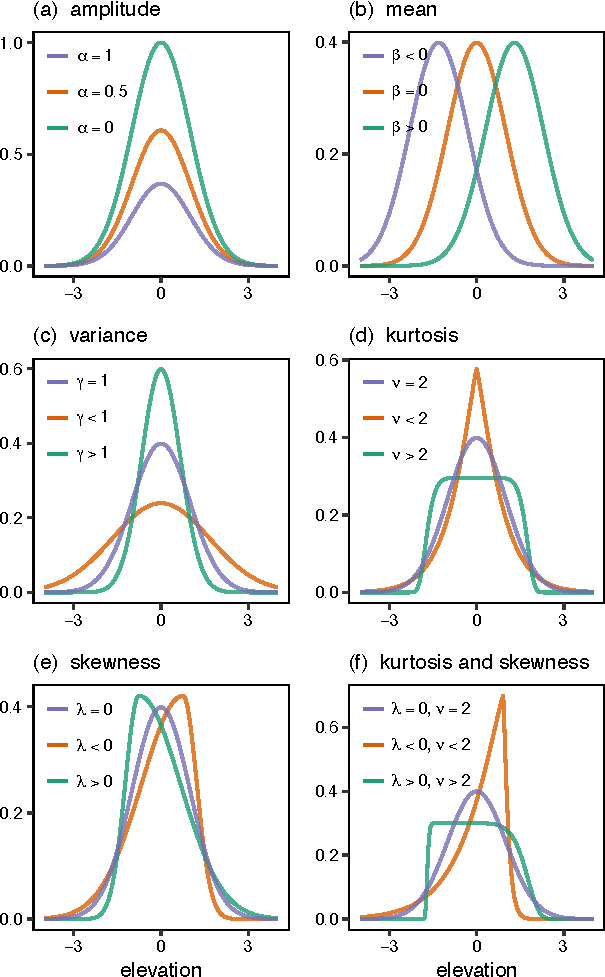
\includegraphics[width=0.9\textwidth]{figures/figure1}
    	  \vspace{0.3cm}
	   \caption{Relationship between mean and variance of species' distributions. These are the results for the main axis of variation for the climatic data (results for the second axis of variation presented in the Supplementary Fig.~2).}
      \label{fig:correlation}
\end{figure}

\begin{figure}[h]
  \centering
    \vspace{0.5cm}
    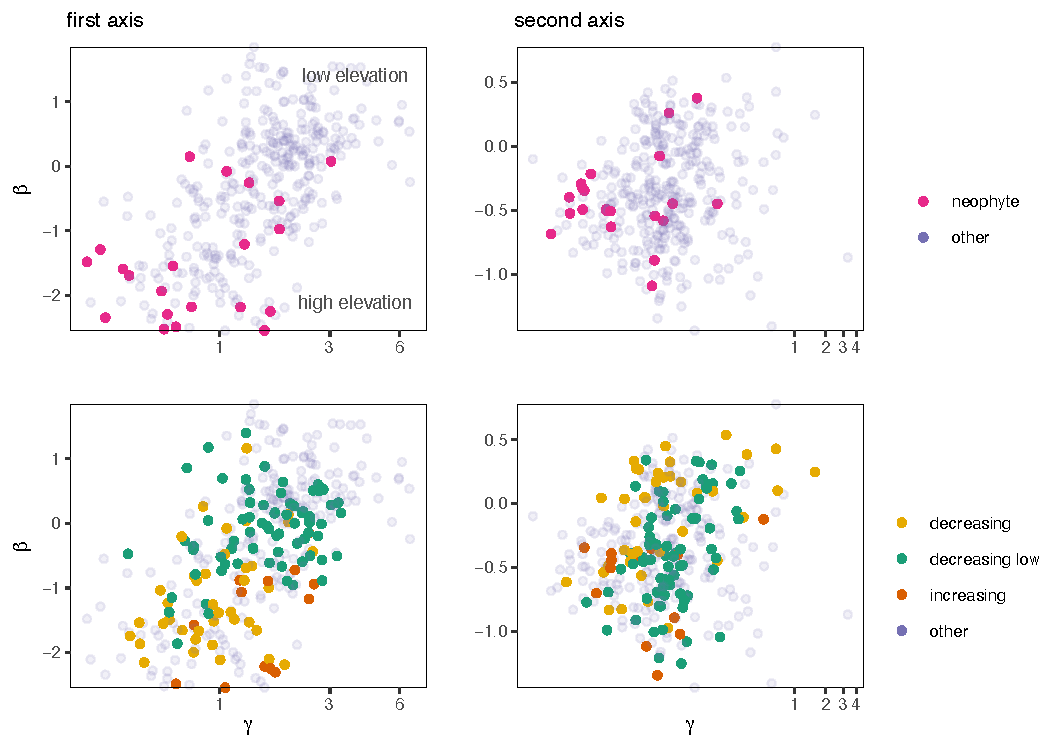
\includegraphics[width=0.9\textwidth]{figures/invasive}
    	  \vspace{0.3cm}
	   \caption{Are there clear geographical patterns for neophytes and for species with decreasing or increasing abundance?}
      \label{fig:neophytes}
\end{figure}

%\section*{Discussion}
\clearpage
\bibliography{references2}

\end{document}
